%%% LaTeX Template: Two column article
%%%
%%% Source: http://www.howtotex.com/
%%% Feel free to distribute this template, but please keep to referal to http://www.howtotex.com/ here.
%%% Date: February 2011

%%% Preamble
\documentclass[DIV=calc,%
              paper=a4,%
              fontsize=11pt,%
              onecolumn]{scrartcl}              % KOMA-article class

\usepackage{lipsum}                          % Package to create dummy text

\usepackage[italian]{babel}                    % Italian language/hyphenation
\usepackage[utf8]{inputenc}
\usepackage[protrusion=true,expansion=true]{microtype}        % Better typography
\usepackage{amsmath,amsfonts,amsthm}          % Math packages
\usepackage[pdftex]{graphicx}                  % Enable pdflatex
\usepackage[svgnames]{xcolor}                  % Enabling colors by their 'svgnames'
\usepackage[hang, small,labelfont=bf,up,textfont=it,up]{caption}  % Custom captions under/above floats
\usepackage{epstopdf}                        % Converts .eps to .pdf
\usepackage{subfig}                          % Subfigures
\usepackage{booktabs}                        % Nicer tables
\usepackage{fix-cm}                          % Custom fontsizes



%%% Custom sectioning (sectsty package)
\usepackage{sectsty}                          % Custom sectioning (see below)
\allsectionsfont{%                              % Change font of al section commands
  \usefont{OT1}{phv}{b}{n}%                    % bch-b-n: CharterBT-Bold font
  }

\sectionfont{%                                % Change font of \section command
  \usefont{OT1}{phv}{b}{n}%                    % bch-b-n: CharterBT-Bold font
  }



%%% Headers and footers
\usepackage{fancyhdr}                        % Needed to define custom headers/footers
  \pagestyle{fancy}                            % Enabling the custom headers/footers
\usepackage{lastpage}

% Header (empty)
\lhead{}
\chead{}
\rhead{}
% Footer (you may change this to your own needs)
\lfoot{\footnotesize \texttt{Progetto di Sistemi Intelligenti} \textbullet ~A.A. 2011/2012}
\cfoot{}
\rfoot{\footnotesize pagina \thepage\ di \pageref{LastPage}}
\renewcommand{\headrulewidth}{0.0pt}
\renewcommand{\footrulewidth}{0.4pt}



%%% Creating an initial of the very first character of the content
\usepackage{lettrine}
\newcommand{\initial}[1]{%
     \lettrine[lines=3,lhang=0.3,nindent=0em]{
            \color{DarkGoldenrod}
            {\textsf{#1}}}{}}



%%% Title, author and date metadata
\usepackage{titling}                              % For custom titles

\newcommand{\HorRule}{\color{DarkGoldenrod}%      % Creating a horizontal rule
                      \rule{\linewidth}{1pt}%
                    }

\pretitle{\vspace{-30pt} \begin{flushleft} \HorRule
        \fontsize{50}{50} \usefont{OT1}{phv}{b}{n} \color{DarkRed} \selectfont
        }
\title{Progetto di \\ Sistemi Intelligenti}          % Title of your article goes here
\posttitle{\par\end{flushleft}\vskip 0.5em}

\preauthor{\begin{flushleft}
          \large \lineskip 0.5em \usefont{OT1}{phv}{b}{sl} \color{DarkRed}}
\author{F. Disperati, D. Pellegrino, N. Redini, }                      % Author name goes here
\postauthor{\footnotesize \usefont{OT1}{phv}{m}{sl} \color{Black}
          University of Pisa                   % Institution of author
          \vskip 1em
          Anno Accademico 2011/2012
          \par\end{flushleft}\HorRule}

\date{}                                        % No date

\begin{document}

\maketitle
\clearpage

\tableofcontents
\clearpage

\section{Introduzione}
\subsection{Analisi del problema}
% The first character should be within \initial{}
\initial{I}l progetto consiste nell'applicazione delle tecniche di Computational Intelligence alla predizione dei consumi energetici di un edificio, adibito ad uffici, relativamente all'impianto di illuminazione.

Lo scopo è quello di predire l'andamento dei consumi e della luminosità all'interno di un edificio implementando quattro diverse tecniche di computational intelligence.

I dati raccolti sono stati sistemati in forma tabellare e riguardano i consumi registrati in 30 giorni tra maggio/giugno 2005. In particolare un singolo campione è costituito da:

\begin{itemize}
  \item Giorno
  \item Mese
  \item Anno
  \item Ora
  \item Minuto
  \item Irraggiamento solare esterno dall'edificio
  \item Luminosità rilevata nell'ambiente monitorato
  \item Energia media consumata
  \item Tipo di giorno (lavorativo/festivo)
\end{itemize}

La luminosità interna viene misurata in $Lux$ ed è stata monitorata attraverso un sensore, l’irraggiamento solare viene rappresentato in $W/m^2$ ed indica la quantità di radiazione solare per unità di superficie; infine l'energia consumata è espressa in $W/h$.


\subsection{Analisi dei dati}
Dal momento che le tecniche che andremo ad analizzare richiedono delle particolari strutture in ingresso, il primo passo è dunque lo studio dei dati forniti atto all'ottimizzazione della struttura interna del modello.

Per prima cosa è doveroso far presente che nei dati è presente un errore nel sample inerente al 30 maggio ( un lunedì ); infatti come è possibile vedere dai dati, tale giorno è marcato come festivo.

Si è dapprima supposto che si trattasse di una qualche festività ( ad esempio il 30 maggio ricorreva il Memorial Day negli U.S.A. ), ma osservando i dati di consumo rilevati, si è subito capito che si trattava semplicemente di un errore.

Un primo possibile approccio risolutivo poteva essere quello di correggere a mano l'errore, bensì vedremo a breve come è stato affrontato il problema.

Osservando i dati si nota che l'anno in questione non cambia ( sono stati campionati solo due mesi ), è dunqe plausibile pensare che l'ingresso 'Anno' non influenzi l'output delle reti che andremo a modellare, e che quindi sia del tutto superfluo; motivo per cui è stato rimosso.

Inoltre, per migliorare le performances delle reti modellate, i dati sono stati mediati con steps di un ora, elimimando quindi anche l'ingresso Minuti; in questo modo gli effetti sulla rete di eventuali picchi anomali (tra i dati campionati) vengono attenuati.

Infine si è scelto di suddividere i due mesi in settimane ( da 1 a 8 ) ed i giorni in “giorni setttimanali” ( da 1 a 7 ); così facendo è stato possibile eliminare l'ingresso 'Tipo di giorno'.

Quest'ultima operazione è stata possibile secondo la seguente considerazione: se il giorno è festivo (sabato o domenica) i consumi energetici sono pressochè nulli, cosa che non accade quando il giorno è lavorativo ( da lunedi a venerdi). 

In sostanza abbiamo trasportato l'informazione che forniva l'ingresso 'Tipo di giorno' al numero di giorno della settimana; sarà poi compito della rete apprendere l'andamento dei consumi durante la settimana; così facendo è stato inoltre possibile correggere l'errore presente nei dati senza intervenire a mano.

Infine è importante notare che l'ingresso 'Tipo di giorno' non sarebbe divenuto inutile qualora nei mesi campionati fossero state presenti festività particolari ( Natale, Pasqua etc ).

Quanto fin'ora descritto è stato reso possibile attraverso lo script ruby sotto riportato.

\inputminted[linenos=true,fontsize=\footnotesize]{ruby}{../../data/conform.rb}
\captionof{listing}{data/conform.rb}


\clearpage


\section{Modelli di fitting}
\subsection{Rete neurale statica}
Il primo strumento che abbiamo utilizzato per lo studio del nostro modello si basa sulle reti di apprendimento di tipo neurale statiche, ovvero il tool Neural fitting di matlab.

Tale tool mette a disposizione dell'utente una semplice GUI la quale permette, attraverso pochi semplici passi di setup, la crezione di una rete neurale statica.

Nonostante tale procedimento sia estramemente semplice, i risultati desiderati possono essere ricavati dopo molte prove dovute a successivi allenamenti della rete ( fase di addestramento ) e a cambiamenti nella struttura interna quali ad esempio il numero di neuroni nascosti.

In particolare la fase di addestramento di una rete neurale prevede che la rete prenda in ingresso un vettore di inputs e ristituisca un risultato, il quale sarà confrontato quindi con un vettore “obiettivo” per verificarne la bontà dei valori ottenuti.

In base all’esito del confronto questa elaborazione viene ripetuta, modificando opportunamente i pesi su ciascun neurone, fino ad ottenere un livello di apprendimento accettabile.

Al fine di ottenere un apprendimento soddisfacente, ovvero che minimizzi l’errore dato dalla differenza tra il vettore obiettivo e il vettore dei risultati ed una retta di regressione il più possibile vicina all'unità, è stato deciso di creare uno script ed una funzione matlab per rendere la ricerca di una rete considerata “ottima” un processo automatico.

Prima di procedere con la spiegazione di tali scripts, è doveroso mostrare quale struttura è stata utilizzata per modellare la rete neurale.

Come possiamo vedere dalla figura sottostante essa prevede uno strato nascosto, composto in linea generale da un numero di neuroni impostabile dall'utente (12 nell'esempio), con funzione di attivazione sigmoide ed uno strato lineare di uscita.\\

\vspace{20px}
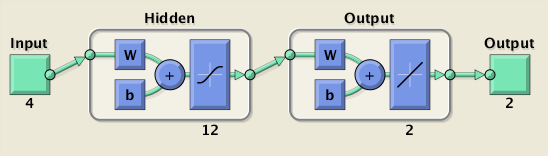
\includegraphics[scale=0.5]{images/neural_net/net.png}
\captionof{figure}[One figure]{Modello di rete neurale}
\vspace{20px}

\subsubsection{Ricerca della migliore rete neurale}
Nell'ottica di automatizzare il processo di modellizzazione della rete, è stata definita sia una funzione per la ricerca di una rete neurale statica considerata ottima, sia uno script per la visualizzazione dei risultati ottenuti.

\paragraph{Funzione searchBestFitting}
Essa provvede alla creazione di una rete neurale al suo addestramento, e all'estrazione dei parametri di interesse quali il coefficiente della retta di regressione ( nel caso test ) e le performances ( valutate sull'MSE ).

La funzione inizializza, e quindi allena, la rete neurale RETRAIN\_ATTEMPTS volte e restituisce alla fine la migliore rete trovata: ovvero quella che ha presentato nella fase di test i migliori parametri.

Chiaramente sono stati impostati anche due GOALs oltre cui la rete ricavata è considerata ottima, nello specifico si consiedera una rete ottima se i valori di regressione sono maggiori o uguale a 0.99 ed MSE minore di 1000.

Ad ogni passo i parametri discriminanti per la bontà della rete sono quelli della fase di test in quanto indicanti la capacità della rete di generalizzare, e dunque di aver correttamente appreso.

E' importante notare che dopo ogni RETRAIN\_ATTEMPTS la struttura interna della rete viene modificata variando il numero di neuroni dello strato nascosto, in modo da confrontare tra loro diverse configurazioni; infine la funzione di addestramento utilizzata è quella standard di backpropagation di Levenberg-Marquardt (trainlm).

La funzione appena esposta è la seguente:

\inputminted[linenos=true,fontsize=\footnotesize]{matlab}{../../src/neural\ network/functions/searchBestFitting.m}
\captionof{listing}{src/neural network/functions/searchBestFitting.m}


\paragraph{Script netfit}
Tale script si occupa semplicemente di inizalizzare il vettori inputs/outputs, richiamare la funzione appena illustrata e quindi stampare a schermo i risultati ottenuti.

In questo script viene inoltre fatto uso della funzione {\bf unix} di matlab per eseguire lo sript conform.rb per la creazione dei dati necessari alla funzione searchBestFitting.

\inputminted[linenos=true,fontsize=\footnotesize]{matlab}{../../src/netfit.m}
\captionof{listing}{src/netfit.m}


\subsubsection{Risultati}
I risultati ottenuti eseguendo lo script sono i seguenti:\\
\vspace{20px}

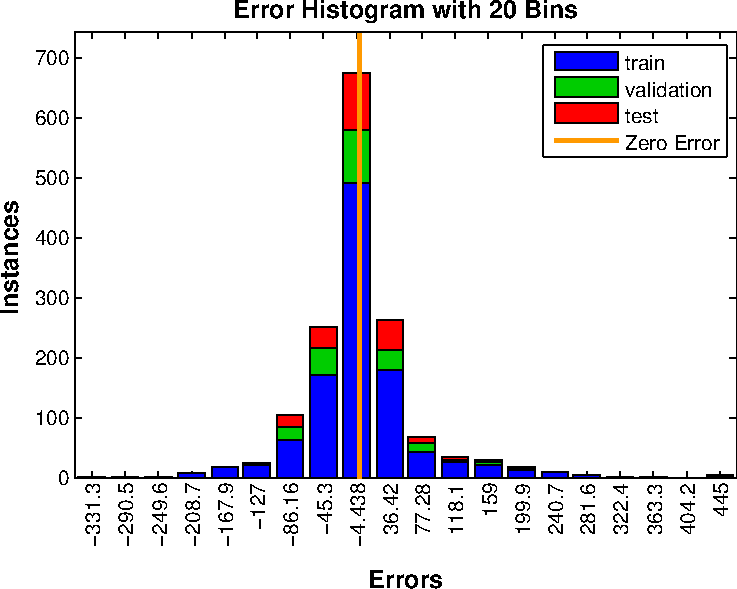
\includegraphics[scale=0.7]{images/neural_net/histogram.pdf}
\captionof{figure}[One figure]{Istogramma degli errori}
\vspace{20px}

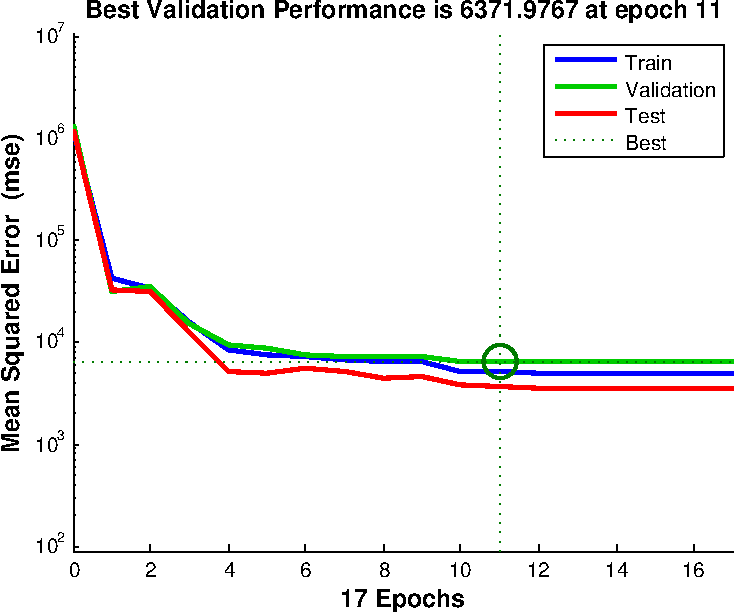
\includegraphics[scale=0.7]{images/neural_net/performances.pdf}
\captionof{figure}[One figure]{Prestazioni della rete (MSE)}
\vspace{20px}

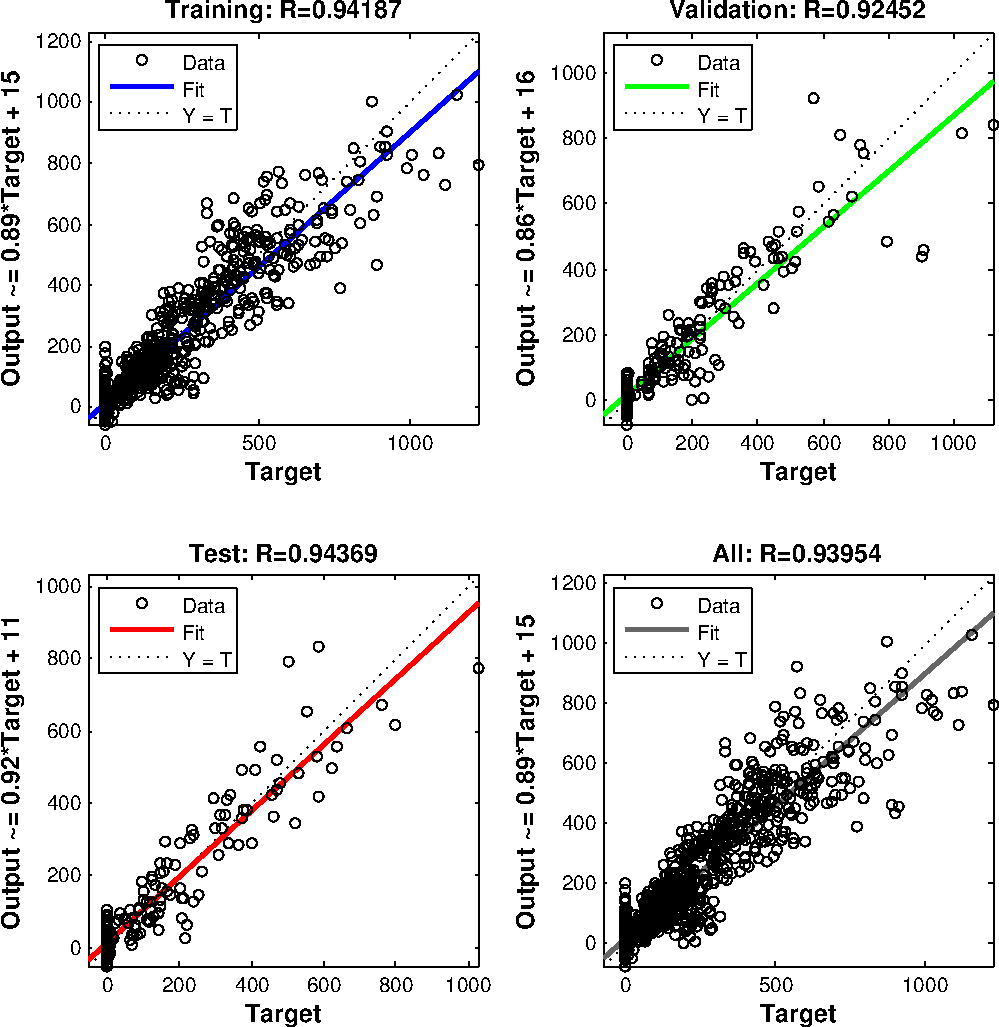
\includegraphics[scale=0.7]{images/neural_net/regressions.pdf}
\captionof{figure}[One figure]{Rette di regressione}
\vspace{20px}

\clearpage




%% FIXME: REMOVE ME!
\begin{table}
\caption{Random table}
\centering
	\begin{tabular}{llr}
		\toprule
		\multicolumn{2}{c}{Name} \\
		\cmidrule(r){1-2}
			First name & Last Name & Grade \\
		\midrule
			John & Doe & $7.5$ \\
			Richard & Miles & $2$ \\
		\bottomrule
	\end{tabular}
\end{table}

\begin{description}
	\item[First] This is the first item
	\item[Last] This is the last item
\end{description}

\end{document}
